\chapter{System Identification Results for Tension Controller} \label{apdx:sysid_kt}

Following the approach described in \ref{ch:sysid:case}, we first assume the OE structure. The grid search process over orders $[n_a, n_b, n_k]$ subject to constraints in \eqref{eqn:oe_bounds} returns the highest performing candidate models as follows,

\begin{table}[h]
    \centering
    \begin{tabular}{r|cccc}
         & Model 1 & Model 2 & Model 3 & Model 4 \\ \hline
         No. of good subbatches & 249 & 259 & 255 & 259 \\
         Average accuracy & 55.62 & 54.38 & 52.75 & 51.89 \\
         Orders & \texttt{[9,10,4]} & \texttt{[10,10,3]} & \texttt{[4,5,4]} & \texttt{[6,7,4]} \\ \hline
    \end{tabular}
    \caption{Results of OE search for tension controller.}
    \label{tab:kt_oe}
\end{table}

As previously addressed in Section \ref{ch:sysid:proc:order}, a high order fit would lose its reliability and robustness, despite its marginally better performance. Therefore Model 3 was selected to generate the ensemble model, which has the following characteristic polynomials, 
\begin{equation*}
    \begin{split}
        B(q) & = 0.02128 q^{-4} - 0.04466 q^{-5} + 0.06583 q^{-6} - 0.04242 q^{-7} \\            
        F(q) & = 1 - 0.4937 q^{-1} - 0.1593 q^{-2} - 0.8731 q^{-3} + 0.2688 q^{-4} + 0.2573 q^{-5}
    \end{split}
\end{equation*}

Similarly, assuming the ARMAX structure, the grid search returns the following candidate models, 
\begin{table}[ht]
    \centering
    \begin{tabular}{r|cccc}
         & Model 1 & Model 2 & Model 3 & Model 4 \\ \hline
         No. of good subbatches & 216 & 215 & 212 & 209 \\
         Average accuracy & 49.24 & 51.27 & 50.20 & 50.28 \\
         Validation average fit & 72.15 & 71.73 & 71.44 & 72.24 \\
         Orders & \texttt{[4,3,3,4]} & \texttt{[4,4,3,4]} & \texttt{[3,4,4,4]} & \texttt{[3,2,2,3]} \\ \hline
    \end{tabular}
    \caption{Results of ARMAX search for tension controller.}
    \label{tab:kt_armax}
\end{table}

Inspecting all candidate models, Model 4 was selected since it slightly outperforms Model 1 in the average fit percent to validation data; Thus, it is also the model of choice used in the closed-loop simulation. The characteristic polynomials are identified as follows, 
\begin{equation*}
    \begin{split}
        A(q) & = 1 - 0.6357 q^{-1} - 0.3797 q^{-2} + 0.01532 q^{-3}\\
        B(q) & = 3.299\times 10^{-4} q^{-3} - 2.847\times 10^{-4} q^{-4}\\
        C(q) & = 1 - 0.3122 q^{-1} - 0.2831 q^{-2}\\
    \end{split}
\end{equation*}

The selected model is similarly validated; Figure \ref{fig:sysid_validate_kt} illustrates the time-domain, frequency-domain, and residual analyses involved. Although the signals are corrupted by noise, the model performance are satisfactory in all metrics indicated per Section \ref{ch:sysid:case:val}.

\begin{figure}
    \centering
    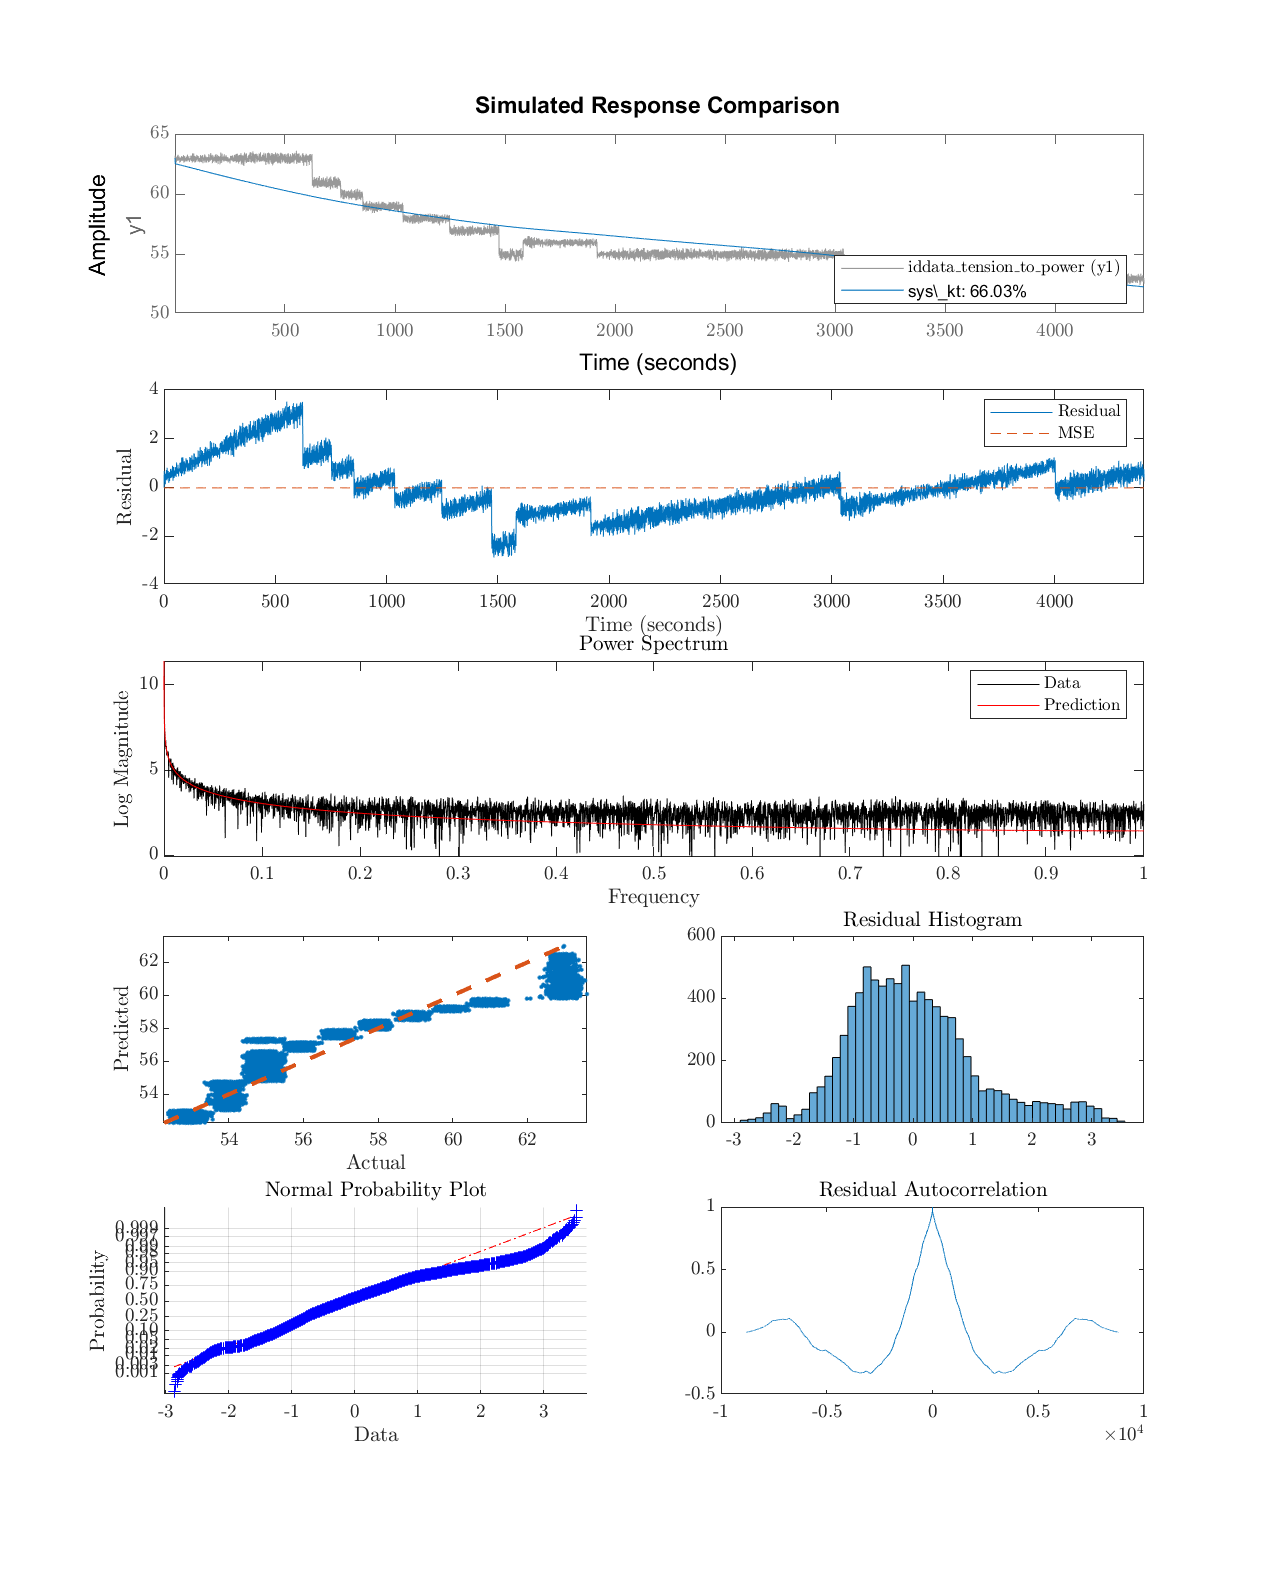
\includegraphics[width=\textwidth]{figures/sysid_validate_kt.png}
    \caption{Time-domain, frequency-domain, and residual analyses performed to validate the ARMAX model for the tension controller.}
    \label{fig:sysid_validate_kt}
\end{figure}